\begin{qu}[Fuse and bulb]\num
Electrical fuses are discussed in the text, without an explicit circuit diagram.
They work by heating to the point where they melt, opening the circuit.
The schematic symbol for a fuse is \includegraphics{electromagnetism/figs/fuse-symbol}.
Logically, which of the following arrangements would protect the
lightbulb from being burned out?

\vspace{20mm}

\includegraphics{electromagnetism/figs/fuse-and-bulb}
\end{qu}
